\documentclass[twoside]{mfitjournal}
\usepackage{amsbib}
\usepackage[T2A]{fontenc}
\usepackage[utf8]{inputenc}
\usepackage[russian]{babel}
\usepackage{graphicx}
\usepackage{amsmath,amssymb}
\usepackage{booktabs}
\usepackage{array}
\usepackage{longtable}
\usepackage{caption}
\usepackage{indentfirst}

\clubpenalty=10000
\widowpenalty=10000
\newcommand{\MFITnumber}{}
\newcommand{\MFITom}{}
\newcommand{\MFITyear}{}
\newcommand{\ISSN}{}
\newcommand{\OISSN}{}
\newcommand{\DOI}{}
\renewcommand{\firstpage}{}
\renewcommand{\lastpage}{}
\SECC{}
\ESECC{}
\captionsetup{labelsep=period}
\newcommand{\degree}{\ensuremath{^\circ}}
\setlength{\headheight}{15pt}

\begin{document}

\rustitle{Лабораторная работа 4.4.2. Фазовая дифракционная решетка}
\shorttitle{Фазовая дифракционная решетка}
\author{Иванов Е.\,С.}
\shortauthor{Иванов Е.\,С.}
\institute{МФТИ, группа Б05-407}
\email{E-mail:}{}
\rcopyr{Иванов Е.\,С.}

\makeatletter
\renewcommand{\tit}{}
\renewcommand{\@oddhead}{}
\renewcommand{\@evenhead}{}
\makeatother

\pagestyle{fancy}
\fancyhf{}
\fancyhead[RE]{Иванов Е.\,С.}
\fancyhead[LO]{Лабораторная работа 4.4.2}
\cfoot{\arabic{page}}

\maketitle

\section*{Цель работы}
Изучение спектра ртутной лампы с помощью фазовой дифракционной решетки при углах падения $22.5\degree$, $45\degree$ и $60\degree$. Определение периода решетки и оценка угловой дисперсии по желтому дублету?

\section*{Оборудование и установка}
Гониометр Г5, эшелетт, ртутная лампа.

\section*{Краткая теория}
Для фазовой дифракционной решетки условие максимумов имеет вид
\begin{equation}
d\bigl(\sin\varphi_m-\sin\psi\bigr)=m\lambda,
\label{eq:grating}
\end{equation}
где $d$ --- период решетки, $\psi$ --- угол падения, $\varphi_m$ --- угол дифракции, $m$ --- порядок спектра, $\lambda$ --- длина волны.

Угловая дисперсия определяется формулой
\begin{equation}
D=\frac{d\varphi}{d\lambda}=\frac{m}{d\cos\varphi_m}.
\label{eq:dispersion}
\end{equation}

Дисперсионная область для соседних порядков:
\begin{equation}
\Delta\lambda=\frac{\lambda}{m}.
\label{eq:interval}
\end{equation}

Для вычисления угла скоса используется соотношение
\begin{equation}
2d\sin\Omega=m_p\lambda_p,
\label{eq:blaze}
\end{equation}
При $m_p=1$ и $\lambda_p=500$ нм угол скоса можно определить после выбора
периода решетки.

\section*{Методика измерений}
В журнале имеются три серии наблюдений при реальных углах падения $22.5\degree$, $45\degree$ и $60\degree$. Для каждой серии выделены нулевой порядок и хорошо различимые линии ртути: фиолетовая, синяя, голубая, зеленая и желтый дублет.

\section*{Обработка результатов}
Положение нормали к решетке определялось по нулевому порядку:
\[
\alpha_{\text{норм}} = 180\degree + \psi.
\]
После этого для каждого наблюдения вычислялись
\[
\varphi = \left| \alpha - \alpha_{\text{норм}} \right|,
\qquad
x=\sin\varphi-\sin\psi,
\]
где $\alpha$ --- отсчет зрительной трубы. По формуле~\eqref{eq:grating} для каждой линии находился период
\[
d_i=\frac{m\lambda_i}{|x_i|}.
\]

\begin{longtable}{@{}llrrp{4.5cm}@{}}
\caption{Линии первого порядка, использованные в аппроксимации}
\label{tab:first_order_points}\\
\toprule
Цвет & $\psi$, \degree & $\sin\varphi-\sin\psi$ & $\lambda$, нм & Заметка \\ \midrule
\endfirsthead
\toprule
Цвет & $\psi$, \degree & $\sin\varphi-\sin\psi$ & $\lambda$, нм & Заметка \\ \midrule
\endhead
\bottomrule
\endfoot
Фиолетовая & 22.5 & 0.24664 & 404.7 & самая яркая \\
Фиолетовая & 22.5 & 0.24777 & 404.7 & вторая, тусклая \\
Синяя & 22.5 & 0.25787 & 435.8 & --- \\
Голубая & 22.5 & 0.29718 & 491.6 & самая яркая \\
Зеленая & 22.5 & 0.32648 & 546.1 & самая яркая \\
Жёлтая 2 & 22.5 & 0.34867 & 577.0 & жёлтый дублет \\
Жёлтая 1 & 22.5 & 0.35065 & 579.1 & жёлтый дублет \\
Фиолетовая & 45 & -0.24536 & 404.7 & --- \\
Синяя & 45 & -0.26612 & 435.8 & --- \\
Голубая & 45 & -0.30037 & 491.6 & --- \\
Зеленая & 45 & -0.33250 & 546.1 & --- \\
Жёлтая 1 & 45 & -0.35418 & 579.1 & жёлтый дублет \\
Жёлтая 2 & 45 & -0.35963 & 577.0 & жёлтый дублет \\
Фиолетовая & 60 & -0.24579 & 404.7 & самая яркая \\
Синяя & 60 & -0.26654 & 435.8 & самая яркая \\
Голубая & 60 & -0.30082 & 491.6 & самая яркая \\
Зеленая & 60 & -0.33241 & 546.1 & --- \\
Жёлтая 1 & 60 & -0.35099 & 579.1 & жёлтый дублет \\
Жёлтая 2 & 60 & -0.35348 & 577.0 & жёлтый дублет \\
\end{longtable}

\begin{figure}[h]
\centering
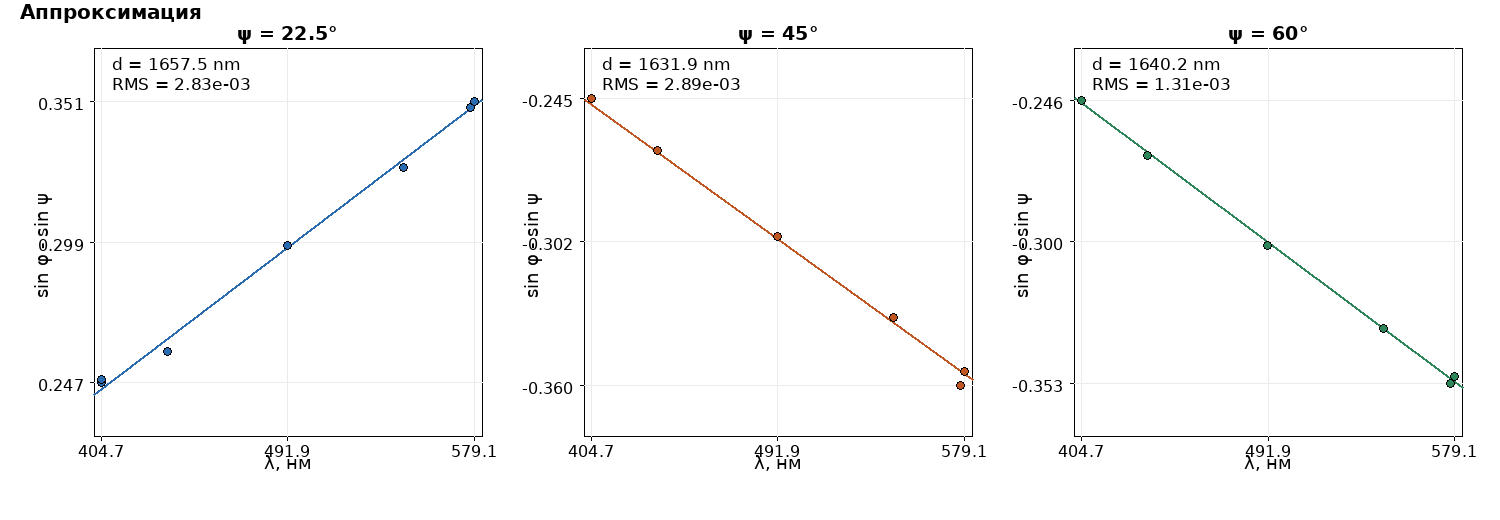
\includegraphics[width=0.98\linewidth]{fig_first_order_fit.png}
\caption{Аппроксимация данных первого порядка}
\end{figure}

\begin{table}[h]
\centering
\caption{Период решетки по отдельным сериям}
\begin{tabular}{@{}lrrr@{}}
\toprule
Серия & $d$, \,$\mu$m & Число точек & RMS остатка по $x$ \\ \midrule
$22.5\degree$ & 1.6575 & 7 & 0.00283 \\
$45\degree$ & 1.6319 & 6 & 0.00289 \\
$60\degree$ & 1.6402 & 6 & 0.00131 \\
\bottomrule
\end{tabular}
\end{table}

\begin{table}[h]
\centering
\caption{Сводка индивидуальных оценок периода по линиям первого порядка}
\begin{tabular}{@{}lrrr@{}}
\toprule
Серия & Число точек & $\langle d \rangle$, \,$\mu$m & $\sigma_d$, \,$\mu$m \\ \midrule
$22.5\degree$ & 7 & 1.6568 & 0.0191 \\
$45\degree$ & 6 & 1.6343 & 0.0155 \\
$60\degree$ & 6 & 1.6401 & 0.0073 \\
\bottomrule
\end{tabular}
\end{table}

Совместная аппроксимация всех $19$ точек первого порядка дает
\[
d = (1.6436 \pm 0.0040)\,\mu\text{m},
\]
где указана стандартная ошибка коэффициента линейной аппроксимации. Как
проверку устойчивости обработки, по средним значениям трех серий первого
порядка получаем
\[
d = (1.643 \pm 0.013)\,\mu\text{m}.
\]
Тем самым статистическая ошибка совместного фита мала, а основной вклад в
разброс результата дает различие между отдельными сериями измерений.

Если принять паспортное значение периода эшелетта
\[
d_{\text{пас}} = \frac{1}{0.65} = 1.538\,\mu\text{m},
\]
то полученное по измерениям значение оказывается больше примерно на $6.9\%$.
Подставляя паспортный период в формулу~\eqref{eq:blaze}, получаем
\[
\Omega = \arcsin\left(\frac{m_p\lambda_p}{2d_{\text{пас}}}\right)
= \arcsin\left(\frac{500}{2\cdot1538}\right)\approx 9.35\degree.
\]
Если использовать экспериментальное значение периода
$d=(1.6436\pm0.0040)\,\mu\text{m}$, то получается близкая оценка
$\Omega \approx 8.75\degree$.

\section*{Угловая дисперсия}
\begin{table}[h]
\centering
\caption{Угловая дисперсия по желтому дублету}
\begin{tabular}{@{}lrrrr@{}}
\toprule
$\psi$, \degree & Порядок $m$ & $\Delta\varphi$, \degree & $D_{\text{exp}}$, мрад/нм & $D_{\text{th}}$, мрад/нм \\ \midrule
$22.5\degree$ & 1 & 0.1667 & 1.385 & 0.894 \\
$45\degree$ & 1 & 0.3333 & 2.770 & 0.650 \\
$45\degree$ & 2 & 0.1667 & 1.385 & 1.217 \\
$60\degree$ & 1 & 0.1667 & 1.385 & 0.709 \\
$60\degree$ & 2 & 0.1667 & 1.385 & 1.234 \\
$60\degree$ & 3 & 0.1667 & 1.385 & 1.856 \\
\bottomrule
\end{tabular}
\end{table}

Для желтого дублета ртути экспериментальная угловая дисперсия лежит в диапазоне
\[
D_{\text{exp}}\sim (1.39\text{--}2.77)\,\text{мрад/нм},
\]
где нижняя и верхняя границы взяты как минимальное и максимальное значения из
таблицы выше. По порядку величины верно.

\section*{Обсуждение результатов}
Все три серии дают согласованный период решетки порядка $1.64\,\mu$m, что соответствует плотности штрихов около $610$ мм$^{-1}$. Разброс между сериями невелик и объясняется конечной точностью углового отсчета.

Индивидуальные оценки периода по линиям первого порядка также согласуются
между собой: их средние значения для трех серий лежат в диапазоне
$1.634$--$1.657\,\mu$m, а характерного систематического дрейфа с длиной волны
не наблюдается.

Первая серия обработана именно как серия при $22.5\degree$. При измерениях была допущена ошибка, которая привела к замене измерений $30\degree$ на $22.5\degree$.

По имеющимся данным можно надежно определить период решетки, а вот оценить
угловую дисперсию по желтому дублету точно не удалось.

\section*{Заключение}
По обработке измерений получен период фазовой дифракционной решетки
\[
d=(1.6436\pm0.0040)\,\mu\text{m},
\]
а разброс средних значений между сериями первого порядка составляет около
$0.013\,\mu$m.
По порядку величины угловая дисперсия желтого дублета согласуется с
теоретической оценкой.

\begin{thebibliography}{9}
\bibitem{handbook}
Лабораторный практикум по общей физике. Том 2. Оптика. Раздел <<Спектральные приборы>> и работа 4.4.2.
\end{thebibliography}

\end{document}
